\section{Pole Placement}

\subsection{Full State Feedback}
Assuming the internal state of a sytem can be accessed completely, the system can be controlled
with a \textit{reference signal} $r$ (scalar) \textit{scaling vector} $\mathbf{S}$ (column vector) and a static gain $\mathbf{K}$ (row vector):
\begin{center}
    % \includegraphics[width = \linewidth]{full_state.png}
    \usetikzlibrary{shapes,arrows,positioning,calc}

\tikzset{
    block/.style = {draw, fill=white, rectangle, minimum height=3em, minimum width=3em},
    tmp/.style  = {coordinate},
    sum/.style= {draw, fill=white, circle, node distance=1cm},
    input/.style = {coordinate},
    output/.style= {coordinate},
    pinstyle/.style = {pin edge={to-,thin,black}
        }
}


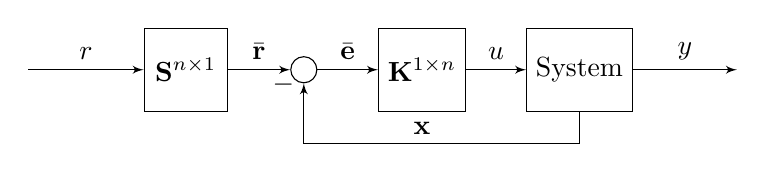
\begin{tikzpicture}[auto, node distance=2cm,>=latex']
    \node [input, name=rinput, node distance=1.5cm]         (rinput)        {};
    \node [block, right of=rinput]                          (scale_vec)     {$\mathbf{S}^{n\times 1}$};
    \node [sum, right of=scale_vec, node distance=1.5cm]    (sum1)          {};
    \node [block, right of=sum1, node distance=1.5cm]       (static_gain)   {$\mathbf{K}^{1\times n}$};
    \node [tmp, below = 0.4cm of static_gain]               (tmp1)          {$\mathbf{x}$};
    \node [block, right of=static_gain]                     (sys)           {System};
    % \node [output, below of=sys] (x) {};
    \node [output, right of=sys, node distance=2cm] (output) {};
    \node at (5,-.75) {$\mathbf{x}$} ;

    \draw [->] (rinput) -- node{$r$} (scale_vec);
    \draw [->] (scale_vec) -- node{$\bar{\mathbf{r}}$} (sum1);
    \draw [->] (sum1) -- node{$\bar{\mathbf{e}}$} (static_gain);
    \draw [->] (static_gain) -- node{$u$} (sys);
    \draw [->] (sys) -- node{$y$} (output);
    \draw [->] (sys) |-(tmp1) -| node[pos=0.99] {$-$} (sum1);
\end{tikzpicture}
\end{center}
%TBD: tikz image with bold vectors to show the dimensions better
The corresponding closed-looop system is
\noindent\begin{align*}
    \dot{\mathbf{x}} & =(\mathbf{A}-\mathbf{BK})\mathbf{x}+\mathbf{B}\bar{N}r, & \bar{N}=\mathbf{KS} \\
    y                & =(\mathbf{C}-\mathbf{DK})\mathbf{x} +\mathbf{D}\bar{N}r
\end{align*}

\subsection{Pole Placement}
Pole placement can be used to tune $\mathbf{K}$ and $\mathbf{S}$ to achieve the desired closed loop poles $\lambda_i$.
The desired characteristic equation is
\noindent\begin{align*}
    \varphi_{cl,des} & =\det{(sI-A+BK)}=(s-\lambda_1)(s-\lambda_2)\ldots(s-\lambda_n) \\
                     & =s^n+\alpha_{n-1}s^{n-1}+\ldots+\alpha_0
\end{align*}

\subsubsection{Reachable Canonical Form}
If the system is in \textbf{reachable canonical form} and $\mathbf{K} = \left[k0,k1,\ldots,k_{n-1}\right]$, then

    {\footnotesize
        \noindent\begin{equation*}
            \mathbf{A}_{\mathrm{cl}}=\mathbf{A-BK}=\begin{bmatrix}
                0        & 1        & \ldots & 0                \\
                0        & 0        & \ldots & 0                \\
                \vdots   & \vdots   & \ddots & 1                \\
                -a_0-k_0 & -a_1-k_1 & \ldots & -a_{n-1}-k_{n-1}
            \end{bmatrix}
        \end{equation*}
    }

and the closed-loop characteristic polynomial can be used to choose the parameters $k_i$ based on the desired parameters $\alpha_i$:
\noindent\begin{align*}
    \varphi(s) & =s^n+(a_{n-1}+k_{n-1})s^{n-1}+\ldots+(a_0+k_0) \overset{!}{=} \varphi_{cl,des} \\
    k_i        & =\alpha_i-a_i,i=0,\ldots,n-1
\end{align*}

\subsubsection{General Case}
If the system is \textbf{controllable} but not in reachable canonical form, the following steps have to be applied
\begin{enumerate}
    \item Similarity transform of $\mathbf{A,B,C,D}$ into reachable canonical form $\mathbf{A',B',C',D'}$:
          \noindent\begin{align*}
              \mathbf{R}' & =\begin{bmatrix}
                                 \mathbf{B}' & \mathbf{A}'\mathbf{B}' & \ldots & {(\mathbf{A}')}^{n-1}\mathbf{B}'
                             \end{bmatrix}
              =\mathbf{TR}                                                                                                \\
              \mathbf{T}  & = \mathbf{R'R}^{-1}
          \end{align*}
    \item Apply method for reachable canonical form
    \item Transform $\mathbf{K}'$ back to the original system:
          \noindent\begin{align*}
              \mathbf{K}^{\prime} & =\left[\alpha_{0}-a_{0},\quad\alpha_{1}-a_{1},\quad\ldots,\quad\alpha_{n-1}-a_{n-1}\right] \\
              \mathbf{K}          & = \mathbf{K'RR}^{-1}
          \end{align*}
\end{enumerate}
\textbf{Remark}
\begin{itemize}
    \item Controllability is a \textbf{necessary and sufficient condition} for arbitrary pole placement.
    \item If the system is diagonalizable but not controllable, the uncontrollable poles can't be moved.
    \item $\mathbf{A'},\mathbf{A}$ share their eigenvalues, therefore a comparison of coefficients can be used.
\end{itemize}

\subsubsection{Ackermann's Formula}
Assuming that the system is \textbf{controllable}, Ackermann's formula can be used to calculate $\mathbf{K}$ for both \textbf{\textit{CT}} and \textbf{\textit{DT}} systems:
\noindent\begin{align*}
    \mathbf{K}               & =\begin{bmatrix}
                                    0, & \ldots, & 0, & 1
                                \end{bmatrix}
    \mathbf{R}^{-1}\varphi_{cl}(\mathbf{A})                                                              \\
    \varphi_{cl}(s)          & =s^n+\alpha_{n-1}s^{n-1}+\ldots+\alpha_0=(s-\lambda_1)\ldots(s-\lambda_n) \\
    \varphi_{cl}(\mathbf{A}) & =\mathbf{A}^n+\alpha_{n-1}\mathbf{A}^{n-1}+\ldots+\alpha_0 I
\end{align*}

\subsubsection{Reference Scaling}
To ensure that the closed-loop systems follows unit steps with zero stedy state error, the scaling vector $\mathbf{S}$ has to be chosen accordingly
\noindent\begin{align*}
    G_{y\rightarrow r}^{cl}(s) & =\mathbf{C}{(s\mathbf{I}-\mathbf{A}+\mathbf{BK})}^{-1}\mathbf{B}\bar{N}r,                                                                                                      & \bar{N}=\mathbf{KS} \\
    G_{y\rightarrow r}^{cl}(0) & \overset{!}{=} 1                                                                                                                                                                                     \\
    \bar{N}                    & =-{\left[\mathbf{C}{(\mathbf{A}-\mathbf{BK})}^{-1}\mathbf{B}\right]}^{-1}                                                                                                                            \\\\
    \bar{N}                    & =\underbrace{\left[\mathbf{CA}^{-1}\mathbf{B}\right]}_{\text{DC ol.}}\cdot\underbrace{{\left[\mathbf{C}{(\mathbf{A}-\mathbf{BK})}^{-1}\mathbf{B}\right]}^{-1}}_{\text{DC cl.}}
\end{align*}
In other words, the scaling vector $\mathbf{S}$ has to be chosen such that $\mathbf{KS}=\bar{N}$.

\subsubsection{MIMO}
\begin{itemize}
    \item If the system is controllable from any one of the inputs, pole placement works.
    \item In addition to the poles, the closed-loop eigenvectors (modal shapes) can be placed
\end{itemize}